\subsection*{Solution to Fall 2012, \#1}
\label{F12Q1}

Suppose $u$ and $v$ are solutions to the PDE, and define $w:=u-v$. Observe that $w$ now satisfies
$$ \left\{
\begin{array}{ll}
	\Delta w = 0 & \text{for} \,\, |x| < 1, \,\, |y| < 1 \\
	w = 0 & \text{for} \,\, |x| = 1, \,\, |y| \leq 1 \\
	w_x = w_y & \text{for} \,\, |y| = 1, \,\, |x| < 1
\end{array}
\right.
$$
There are (at least) two ways of solving this problem --- both will be explained.

The first method uses the maximum principle for harmonic functions. Define
\begin{gather*}
	D := \{ (x,y) \, | \, |x| < 1, \, |y| < 1 \} \\
	\Gamma_1 := \{ (x,y) \, | \, |x|=1, \, |y| \leq 1 \} \\
	\Gamma_2 := \{ (x,y) \, | \, |y|=1, \, |x|<1 \}
\end{gather*}
Note that $\Gamma_1$ contains the corners of the square domain. Because $w$ is harmonic in $D$, the maximum of $w$ must occur on $\d D = \Gamma_1 \cup \Gamma_2$. If the maximum of $w$ occurs on $\Gamma_1$, then $w \leq 0$ in $D$. Now, suppose the maximum of $w$ occurs on $\Gamma_2$ at $(x_0,y_0)$, and furthermore, suppose this is a strict maximum. If not, then, by the strong maximum principle, $w$ is constant on $D$. This would mean $w \equiv 0$ since $w = 0$ on $\Gamma_1$, implying that the solution is unique. So, if $w$ achieves a strict maximum on $\Gamma_2$, then, by Hopf's Lemma,
$$\frac{\d w}{\d y}(x_0,y_0) = \frac{\d w}{\d x}(x_0,y_0) > 0 $$
Note that we can apply Hopf's Lemma here because $\Gamma_2$ satisfies the interior ball property (this is why we chose to let $\Gamma_1$ contain the corners of the domain). However, since $w_x(x_0,y_0)$ is strictly positive, this would imply that $w$ does not achieve its maximum at $(x_0,y_0)$. Thus, by contradiction, if a maximum were to occur on $\Gamma_2$, it can't be a strict maximum, implying that $w \equiv 0$. Hence, we've shown that either $w \leq 0$ or $w \equiv 0$ on $D$.

Swapping the roles of $u$ and $v$ will yield $w \geq 0$ or $w \equiv 0$ on $D$. Therefore, $w \equiv 0$, implying that the solution is unique.

\vspace{0.4cm}

The second method uses integration by parts. Multiplying the PDE by $w$ and integrating both sides yields
\begin{align*}
0 &= \int_D \Delta w w \, dx \\
&= - \int_D |\nabla w|^2 \, dx + \int_{\d D} \frac{\d w}{\d \nu} w \, dSx	
\end{align*}
where $\nu$ is the unit outer normal. Since $w = 0$ on $\Gamma_1$, we only need to worry about $\Gamma_2$. Observe,
\begin{align*}
\int_{\d D} \frac{\d w}{\d \nu} w \, dSx &= \int_{\Gamma_2} \frac{\d w}{\d \nu} w \, dSx \\
&= \int_{1}^{-1} w_y(x,1) w(x,1) \, dx + \int_{-1}^1 -w_y(x,-1) w(x,-1) \, dx
\end{align*}
where the first integral is for the top portion of $\Gamma_2$ and the second integral is for the bottom portion of $\Gamma_2$. Now, we compute
$$ \int_1^{-1} w_y(x,1) w(x,1) \, dx = \int_1^{-1} w_x(x,1) w(x,1) \, dx = \frac{1}{2} \int_1^{-1} (w(x,1)^2))_x \, dx = 0$$
where the last equality is because of the boundary conditions on $w$. Similarly,
$$ \int_{-1}^1 -w_y(x,-1)w(x,-1) \, dx = 0 $$
Hence, we have
$$ 0 = -\int_D |\nabla w|^2 \, dx $$
implying that $u$ is constant in $D$. However, because $w = 0$ on $\Gamma_1$, we have that $w \equiv 0$ in $D$. Therefore, the solution to the PDE is unique. \qed




\subsection*{Solution to Fall 2012, \#2}
\label{F12Q4}

\subsubsection*{Solution to $2a$}

We compute
$$ \frac{d}{dt} \int_{\R^2} \rho(x,t)\, dx = \int_{\R^2} \rho_t(x,t) \, dx = \int_{\R^2} \Delta (\rho^2) + \nabla \cdot (2x \rho) \, dx $$
Observe that, because $\rho$ is compactly supported for all time $t>0$, using integration by parts yields
$$ \int_{\R^2} \Delta (\rho^2) \, dx = 0 $$
Furthermore,
$$ \int_{\R^2} \nabla \cdot (2x \rho) \, dx  = \int_{\R^2} 2n\rho + 2x \cdot \nabla \rho \, dx $$
Then, by integration by parts, the above boils down to
$$ \int_{\R^2} \nabla \cdot (2x \rho) \, dx = \int_{\R^2} 2n \rho - 2n \rho \, dx = 0$$
Again, because $\rho$ is compactly supported for all $t>0$, the boundary terms vanish. Thus,
$$ \frac{d}{dt} \int_{\R^2} \rho(x,t) \, dx = 0 $$
implying that
$$ \int_{\R^2} \rho(x,t) \, dx = \int_{\R^2} \rho(x,0) \, dx = 1 $$
\hfill \qed

\subsubsection*{Solution to $2b$}

Again, we will take a time derivative of the integral.
$$ \frac{d}{dt} \int_{\R^2} \rho^2 + \rho |x|^2 + C \rho \, dx = \int_{\R^2} 2 \rho \rho_t + \rho_t |x|^2 \, dx $$
Note that, because of part (a), $\int_{\R^2} C \rho \, dx = C$, so that term vanishes after taking a time derivative. Continuing with our computations, we have
\begin{align*}
\int_{\R^2} \rho_t(2\rho + |x|^2) \, dx &= \int_{\R^2} \left( \Delta  (\rho^2) + \nabla \cdot (2x \rho) \right) \left( 2\rho + |x|^2 \right) \, dx \\
&= -\int_{\R^2} (\nabla (\rho^2) + 2x \rho) \cdot \nabla (2\rho + |x|^2) \, dx \\
&= -\int_{\R^2} \rho (2 \nabla \rho + 2x) \cdot (2\nabla \rho + 2x) \, dx \\
&= -\int_{\R^2} \rho |2 \nabla \rho + 2x|^2 \, dx \leq 0
\end{align*}
because $\rho$ is assumed to be nonnegative for all time $t>0$. Note, the second inequality is from applying integration by parts. Again, the boundary terms vanish because $\rho$ is compactly supported for all time $t>0$. Hence, the energy is non-increasing for any choice of $C$. (I don't think we have enough to show that the energy is \emph{decreasing}.)

\subsubsection*{Solution to $2c$}

Since the energy is both positive and non-increasing, we know that the energy is either constant or it's decreasing to 0. In both cases, we can make the conclusion that as $t \to \infty$,
$$ \frac{d}{dt} \int_{\R^2} \rho^2 + \rho|x|^2 + C \rho \, dx = -\int_{\R^2} \rho |2 \nabla \rho + 2x|^2 \, dx \to 0$$
This implies that either $\rho \to 0$ or $2 \nabla \rho + 2x \to 0$ as $t \to \infty$. Because of our work in part (a), the first option can't hold, so we have\
\begin{align*}
2 \nabla \rho + 2x \to 0 \quad &\implies \quad \nabla \rho \to -x \\
&\implies \quad \rho \to C_0 -\frac{|x|^2}{2}\
\end{align*}
Because $\rho$ is nonnegative for all time $t>0$, we must have $ \rho \to \left( C_0 - \frac{|x|^2}{2} \right)_+$ as $t \to \infty$. To find $C_0$, we use part (a).
\begin{align*}
\int_{\R^2} \rho(x,t) \, dx = 1 \quad &\implies \quad \int_{\R^2} \left( C_0 - \frac{|x|^2}{2} \right)_+ \, dx = 1 \\
&\implies \quad \int_{B(0,\sqrt{2C_0})} C_0 - \frac{|x|^2}{2} \, dx = 1 \\
&\implies \quad \int_0^{2\pi} \int_0^{\sqrt{2C_0}} \left( C_0 - \frac{r^2}{2} \right) r \, dr d\theta = 1\\
&\implies \quad 2 \pi \left( C_0^2 - \frac{C_0^2}{2} \right) = 1 \\
&\implies \quad C_0 = \frac{1}{\sqrt{\pi}}
\end{align*}
\hfill \qed











\subsection*{Solution to Fall 2012, \#3}
\label{F12Q3}

Letting $v := u'$, we can rewrite the second-order ODE into a first-order system:
\begin{align*}
u' &= v \\
v' &= -f(u) + \lambda v
\end{align*}
Define $F : \R^2 \to \R^2$ as $F(u,v) = (v, -f(u) + \lambda v)$, and observe that
$$ \nabla \cdot F(u,v) = \lambda > 0 $$
Thus, by the Bendixson-Dulac theorem, the ODE has no periodic solutions other than any stationary equilibrium solutions ($u \equiv c \in \R$). \hfill \qed












\subsection*{Solution to Fall 2012, \#4}

Let $u(x, t) = f(x + t)$ with $f$ having a jump discontinuity at $x = x_{0}$ and fix an $v \in C_{0}^{\infty}(\R \times [0, \infty))$. Since we will want to show that
$f(x + t)$ is a weak solution to the wave equation, we will assume $g$ is the weak derivative of $f$.
We have
\begin{align}\label{F124eq1}
\int_{0}^{\infty}&\int_{-\infty}^{\infty}f(x + t)v_{tt}\, dx\, dt = \int_{-\infty}^{\infty}\int_{0}^{\infty}f(x + t)v_{tt}\, dt\, dx\nonumber\\
&= \int_{-\infty}^{\infty}1_{x_{0} - x \geq 0}\int_{0}^{\infty}f(x + t)v_{tt}\, dt\, dx + \int_{-\infty}^{\infty}1_{x_{0} - x < 0}\int_{0}^{\infty}f(x + t)v_{tt}\, dt\, dx\nonumber\\
&= \int_{-\infty}^{x_{0}}\bigg(\int_{0}^{x_{0} - x}f(x + t)v_{tt}\, dt + \int_{x_{0} - x}^{\infty}f(x + t)v_{tt}\, dt\bigg)\, dx + \int_{x_{0}}^{\infty}\int_{0}^{\infty}f(x + t)v_{tt}\, dt\, dx.
\end{align}
Since $v$ is of compact support and
$$\int_{a}^{b}f(x + t)v_{tt}\, dt = f(x + b)v_{t}(x, b) - f(x + a)v_{t}(x, a) - \int_{a}^{b}f'(x + t)v_{t}\, dt,$$
we have that \eqref{F124eq1} is equal to
\begin{equation}
\begin{aligned}\label{F124eq2}
\int_{-\infty}^{x_{0}}&\bigg(f_{-}(x_{0})v_{t}(x, x_{0} - x) - f(x)v_{t}(x, 0) - \int_{0}^{x_{0} - x}f'(x + t)v_{t}\, dt - f_{t}(x_{0})v_{t}(x, x_{0} - x)\\
&\quad\quad\quad - \int_{x_{0} - x}^{\infty}f'(x + t)v_{t}\, dt\bigg)\, dx + \int_{x_{0}}^{\infty}-f(x)v_{t}(x, 0)\, dx - \int_{0}^{\infty}f'(x + t)v_{t}\, dt\, dx\\
&= (f_{-}(x_{0}) - f_{+}(x_{0}))\int_{-\infty}^{x_{0}}v_{t}(x, x_{0} - x)\, dx - \int_{-\infty}^{\infty}f(x)v_{t}(x, 0)\, dx - \int_{0}^{\infty}\int_{-\infty}^{\infty}f'(x + t)v_{t}\, dx\, dt.
\end{aligned}
\end{equation}
Since $v$ is of compact support and
$$\int_{a}^{b}f'(x + t)v_{t}\, dx = f(b + t)v_{t}(b, t) - f(a + t)v_{t}(a, t) - \int_{a}^{b}f(x + t)v_{tx}\, dx$$
we have
\begin{equation}
\begin{aligned}\label{F124eq3}
\int_{0}^{\infty}\int_{-\infty}^{\infty}f'(x + t)v_{t}\, dx\, dt &= \int_{0}^{\infty}\bigg(\int_{-\infty}^{x_{0} - t}f'(x + t)v_{t}\, dx + \int_{x_{0} - t}^{\infty}f'(x + t)v_{t}\, dx\bigg)\, dt\\
&= (f_{-}(x_{0}) - f_{+}(x_{0}))\int_{0}^{\infty}v_{t}(x_{0} - t, t)\, dt - \int_{0}^{\infty}\int_{-\infty}^{\infty}f(x + t)v_{tx}\, dx\, dt.
\end{aligned}
\end{equation}
A change of variables shows that
$\int_{0}^{\infty}v_{t}(x_{0} - t, t)\, dt = \int_{-\infty}^{x_{0}}v_{t}(x, x_{0} - x)\, dx$
and hence combining this with \eqref{F124eq1}-\eqref{F124eq3} yields
\begin{align}\label{F124eq5}
\int_{0}^{\infty}&\int_{-\infty}^{\infty}f(x + t)v_{tt}\, dx\, dt = -\int_{-\infty}^{\infty}f(x)v_{t}(x, 0)\, dx + \int_{0}^{\infty}\int_{-\infty}^{\infty}f(x + t)v_{tx}\, dx\, dt.
\end{align}
We now similarly consider the $v_{xx}$ term. For $t \in [0, \infty)$, note that $x_{0} - t \in (-\infty, \infty)$.
Since
$$\int_{a}^{b}f(x + t)v_{xx}\, dx = f(b + t)v_{x}(b, t) - f(a + t)v_{x}(a, t) - \int_{a}^{b}f'(x + t)v_{x}\, dx,$$
we have
\begin{align*}
\int_{0}^{\infty}\int_{-\infty}^{\infty}f(x + t)v_{xx}\, dx\, dt &= \int_{0}^{\infty}\bigg(\int_{-\infty}^{x_{0} - t}f(x + t)v_{xx}\, dx + \int_{x_{0} - t}^{\infty}f(x + t)v_{xx}\, dx\bigg)\, dt\\
&= (f_{-}(x_{0}) - f_{+}(x_{0}))\int_{0}^{\infty}v_{x}(x_{0} - t, t)\, dt - \int_{0}^{\infty}\int_{-\infty}^{\infty}f'(x + t)v_{x}\, dx\, dt.
\end{align*}
Similarly to the calculations done at the beginning of this solution,
\begin{align*}
\int_{0}^{\infty}\int_{-\infty}^{\infty}&f'(x + t)v_{x}\, dx\, dt = \int_{-\infty}^{\infty}\int_{0}^{\infty}f'(x + t)v_{x}\, dt\, dx\\
&= \int_{-\infty}^{\infty}\bigg(1_{x_{0} - x \geq 0}\int_{0}^{\infty}f'(x + t)v_{x}\, dt + 1_{x_{0} - x < 0}\int_{0}^{\infty}f'(x + t)v_{x}\, dt\bigg)\, dx\\
&= \int_{-\infty}^{x_{0}}\bigg(\int_{0}^{x_{0} - x}f'(x + t)v_{x}\, dt + \int_{x_{0} - x}^{\infty}f'(x + t)v_{x}\, dt\bigg)\, dx + \int_{x_{0}}^{\infty}\int_{0}^{\infty}f'(x + t)v_{x}\, dt\, dx.
\end{align*}
Since
$$\int_{a}^{b}f'(x + t)v_{x}\, dt = f(x + b)v_{x}(x, b) - f(x + a)v_{x}(x, a) - \int_{a}^{b}f(x + t)v_{xt}\, dt,$$
it follows that
\begin{align*}
\int_{0}^{\infty}&\int_{-\infty}^{\infty}f'(x + t)v_{x}\, dx\, dt\\
& = (f_{-}(x_{0}) - f_{+}(x_{0}))\int_{-\infty}^{x_{0}}v_{x}(x, x_{0} - x)\, dx - \int_{-\infty}^{\infty}f(x)v_{x}(x,0)\, dx - \int_{-\infty}^{\infty}\int_{0}^{\infty}f(x + t)v_{xt}\, dt\, dx.
\end{align*}
Again by a change of variables $\int_{0}^{\infty}v_{x}(x_{0} - t, t)\, dt =\int_{-\infty}^{x_{0}}v_{x}(x, x_{0} - x)\, dx$ and hence
\begin{align}\label{F124eq6}
\int_{0}^{\infty}\int_{-\infty}^{\infty}f(x + t)v_{xx}\, dx\, dt = \int_{-\infty}^{\infty}f(x)v_{x}(x, 0)\, dx + \int_{-\infty}^{\infty}\int_{0}^{\infty}f(x + t)v_{xt}\, dt\, dx.
\end{align}
Subtracting \eqref{F124eq6} from \eqref{F124eq5} yields
\begin{align*}
\int_{0}^{\infty}\int_{-\infty}^{\infty}f(x + t)(v_{tt} - v_{xx})\, dx\, dt& = -\int_{-\infty}^{\infty}f(x)v_{t}(x, 0)\, dx - \int_{-\infty}^{\infty}f(x)v_{x}(x, 0)\, dx\\
& = -\int_{-\infty}^{\infty}f(x)v_{t}(x, 0)\, dx + \int_{-\infty}^{\infty}g(x)v(x, 0)\, dx
\end{align*}
where in the last equality we have used that the weak derivative of $f$ is $g$.
This shows that $u(x, t) = f(x + t)$ is a weak solution of the wave equation.
\hfill\qed

\subsection*{Solution to Fall 2012, \#5}
\label{F12Q5}

\subsubsection*{Solution to $5a$}

We convert to polar coordinates. Let $x = r\cos\theta$ and $y = r\sin \theta$. Then,
\begin{align*}
r^2 =x^2 + y^2 \quad &\implies \quad r\dot{r} = x\dot{x} + y \dot{y} \\
&\implies \quad \dot{r} = \dot{x} \cos \theta + \dot{y} \sin \theta \\
&\implies \quad \dot{r} = (-r^{2a+1} \sin \theta) \cos \theta + (r^{2a+1} \cos \theta) \sin \theta \\
&\implies \quad \dot{r} = 0
\end{align*}
and
\begin{align*}
\tan \theta = \frac{y}{x} \quad &\implies \quad (\sec^2 \theta) \dot{\theta} = \frac{x \dot{y} - y \dot{x}}{x^2} \\
&\implies \quad \dot{\theta} = \frac{(r \cos \theta)(r^{2a+1} \cos \theta)+(r \sin \theta)(r^{2a+1} \sin \theta)}{r^2} \\
&\implies \quad \dot{\theta} = r^{2a}
\end{align*}
Hence, we have $r = C$ and $\theta = C^{2a}t + \tilde{C}$ for constants $C$ and $\tilde{C}$. In this case, the trajectories are circles and the system is globally well-posed forward and backward in time as long as don't have both $r(0) = 0$ and $a < 0$. \hfill \qed

\subsubsection*{Solution to $5b$}

This time, going thorugh similar calculations as in part (a), we have
$$\dot{r} = -r^{2a+1} \quad \text{and} \quad \dot{\theta} = 0 $$
Solving the ODEs yield
$$ r^{-2a} = 2at - 2aC \quad \text{and} \quad \theta = \tilde{C} $$
for constants $C$ and $\tilde{C}$.

If $a < 0$, let $b = -a$ (for ease of notation). Then, $r^{2b} = -2bt + 2bC$, implying that
$$ r = \left( 2bC - 2bt \right)^{1/2b}, \quad \text{where} \quad C = \frac{r(0)^{2b}}{2b} = \frac{r(0)^{2|a|}}{2|a|} $$
In this case, the system is globally well-posed backward in time. The system is only locally well-posed forward in time since we can only solve until time
$$ t = C = \frac{r(0)^{2|a|}}{2|a|} $$
before the radius becomes undefined. For this case, as $t \to -\infty$, the trajectory starts from $r=r(0)$ and traces a ray (that starts at the origin and forms an angle of $\theta = \tilde{C}$ with the $x$-axis) out to infinity. As $t \to C^-$, the trajectory starts from $r=r(0)$ and traces the same ray toward the origin. Note that we will actually reach the origin before well-posedness breaks.

If $a > 0$, we have
$$ r = \left( \frac{1}{2at - 2aC} \right)^{1/2a}, \quad \text{where} \quad C = \frac{r(0)^{-2a}}{-2a} $$
In this case, the system is globally well-posed forward in time. The system is only locally well-posed backward in time since we can only solve until time
$$ t = C = \frac{r(0)^{-2a}}{-2a} $$
before the radius blows up. For this case, as $t \to \infty$, the trajectory starts from $r=r(0)$ and traces a ray (that starts at the origin and forms an angle of $\theta = \tilde{C}$ with the $x$-axis) toward the origin, only getting arbitrarily close to the origin. As $t \to C^+$, the trajectory starts from $r=r(0)$ and traces the same ray toward infinity. Because we can only get arbitrarily close to the origin, we also require $r(0) \neq 0$ for this case. \hfill \qed

\subsection*{Solution to Fall 2012, \#6}
\label{F12Q6}

\subsubsection*{Solution to $6a$}

We used generalized method of characteristics to solve this problem, which is analogous to method of characteristics in one dimension. We have
$$
\begin{array}{lll}
\asep
\dot{t}(s) = 1, \quad t(0) = 0 & \implies & t(s) = s \\ \asep
\dot{\vx}(s) = \vz(s), \quad \vx(0) = \vx_0 & \implies & \vx(s) = \vx(t) = \vu_0(\vx_0)t + \vx_0 \\ \asep
\dot{\vz}(s) = 0, \quad \vz(0) = \vu_0(\vx_0) & \implies & \vz(s) = \vz(t) = \vu_0(\vx_0)
\end{array}
$$
Therefore,
$$ \vu(\vx,t) = \vu_0 (\vr) \quad \text{where} \quad \vx = \vu_0(\vr) t + \vr $$
\hfill \qed

\subsubsection*{Solution to $6b$}

We compute
$$ \vu(\vx,t) = \vu_0(\vr) \quad \implies \quad \frac{\d \vu}{\d \vx} = \frac{\d \vu_0}{\d \vx}(\vr) \frac{\d \vr}{\d \vx} $$
and
\begin{align*}
\vx = \vu_0(\vr) t + \vr \quad &\implies \quad \operatorname{Id} = \frac{\d \vu_0}{\d \vx}(\vr) \frac{\d \vr}{\d \vx} t + \frac{\d \vr}{\d \vx} \\
&\implies \quad \frac{\d \vr}{\d \vx} = \left[ \frac{\d \vu_0}{\d \vx}(r) t + \operatorname{Id} \right]^{-1}
\end{align*}
Thus,
$$ \frac{\d \vu}{\d \vx} = \frac{\d \vu_0}{\d \vx} (r) \left[ \frac{\d \vu_0}{\d \vx}(r) t + \operatorname{Id} \right]^{-1} $$
Let $\lambda$ be an eigenvalue of $\frac{\d \vu_0}{\d \vx}$. Then, eigenvalues of $\frac{\d \vu}{\d \vx}$ are of the form $\frac{\lambda}{1 + t\lambda}$. To see this, let $v$ be the corresponding eigenvector to $\lambda$ for $\frac{\d \vu_0}{\d \vx}$. Then,
\begin{align*}
\left[ \frac{\d \vu_0}{\d \vx}(r) t + \operatorname{Id} \right] v = t\lambda v + v = (1 + \lambda t) v \quad &\implies \quad \left(\left[ \frac{\d \vu_0}{\d \vx}(r) t + \operatorname{Id} \right]^{-1} \right)v = (1+\lambda t)^{-1} v \\
&\implies \quad \left(\frac{\d \vu_0}{\d \vx} (r) \left[ \frac{\d \vu_0}{\d \vx}(r) t + \operatorname{Id} \right]^{-1} \right)v = \lambda (1+ \lambda t)^{-1} v
\end{align*}
Since $\left| \frac{\d \vu}{\d \vx} \right| > \rho\left( \frac{\d \vu}{\d \vx} \right)$, where
$$ \rho\left( \frac{\d \vu}{\d \vx} \right) = \max \left\{ \frac{|\lambda|}{|1+t\lambda|} \, : \, \lambda \,\, \text{eigenvalue of} \,\, \frac{\d \vu_0}{\d \vx} \right\}$$
we have finite time blow up of $\left| \frac{\d \vu}{\d \vx} \right|$ if $ \frac{\d \vu_0}{\d \vx} $ has at least one negative eigenvalue. \hfill \qed














\subsection*{Solution to Fall 2012, \#7}
\label{F12Q7}

Suppose $w_n \in X_n$ is the function that minimizes the Rayleigh quotient and $m_n$ is the value of the Rayleigh quotient of evaluateed at $w_n$. That is,
\[
m_n = \frac{||\del w_n||^2}{||w_n||^2}
\]
We first show that $m_n$ is the eigenvalue associated to the function $w_n$. Let $v \in X_n$ be an arbitrary test function, and consider
\[
f(\ep) := \frac{|| \del (w_n+\ep v)||^2}{||w_n+\ep v||^2}
\]
Observe that $f$ has a minimum at $\ep = 0$, which implies that $f'(0) = 0$. Thus, we have
\begin{align*}
\lim_{\ep \to 0} \frac{f(\ep) - f(0)}{\ep} &= \lim_{\ep \to 0} \frac{1}{\ep} \left[ \frac{ || \del w_n||^2 + 2\ep \langle \del w_n, \del v \rangle + \ep^2 ||\del v||^2}{||w_n||^2 + 2\ep \langle w_n, v \rangle + \ep^2 ||v||^2} - \frac{|| \del w_n||^2}{||w_n||^2} \right] \\
&= \frac{2 \langle \del w_n, \del v \rangle ||w_n||^2 - 2 \langle w_n, v \rangle ||\del w_n||^2}{||w_n||^4} = 0
\end{align*}
It then follows that
\begin{align*}
\langle \del w_n, \del v \rangle ||w_n||^2  = \langle w_n,v \rangle ||\del w_n||^2 \quad &\implies \quad  \langle \del w_n, \del v \rangle = m_n \langle w_n, v\rangle \\
&\implies \quad \int_{\Omega} \del w_n \cdot \del v \, dx = m_n \int_{\Omega} w_nv \, dx \\
&\implies \quad -\int_{\Omega} \lap w_n v \, dx = m_n \int_{\Omega} w_nv \, dx
\end{align*}
where the final line above is a result of integration by parts. The boundary terms vanish because of the homogeneous Neumann boundary condition. Hence, for all $v \in X_n$, we have
\[
\int_{\Omega} (\lap w_n + m_n w_n) v \, dx = 0
\]
We now aim to show that the same is true for all test functions $v \in H^1(\Omega)$, Let $v \in H^1(\Omega)$ be an arbitrary test function. Let $g$ be defined so that
\[
g(x) = v(x) - \sum_{k=1}^{n-1} c_k v_k(x), \quad \text{where} \quad c_k = \frac{ \langle v, v_k \rangle}{\langle v_k, v_k \rangle}
\]
where $v_i$ for $i=1, \dots, n-1$ are the first $n-1$ eigenfunctions. Then,
\begin{align}
\notag \int_{\Omega} (\lap w_n + m_n w_n)v \, dx  &= \int_{\Omega} (\lap w_n + m_n w_n) \left( g + \sum_{k=1}^{n-1} c_k v_k \right) \, dx \\
\label{f127eq} &= \int_{\Omega} (\lap w_n + m_n w_n)g\, dx + \int_{\Omega} (\lap w_n + m_n w_n) \left( \sum_{k=1}^{n-1} c_k v_k \right) \, dx
\end{align}
We aim to show that both integrals of \eqref{f127eq} are 0. First, we claim that $\langle g, v_i \rangle = 0$ for $i = 1, \dots, n-1$.
\begin{align*}
\langle g, v_i \rangle &= \langle v - \sum_{k=1}^{n-1} c_k v_k, v_i \rangle \\
&= \langle v, v_i \rangle - \sum_{k=1}^{n-1} c_k \langle v_k, v_i \rangle \\
&= \langle v, v_i \rangle - c_i \langle v_i, v_i \rangle \\
&= 0
\end{align*}
Hence, $g \in X_n$, so by our work above
$$
\int_{\Omega} (\Delta w_n + m_n w_n )g \, dx = 0
$$
Next, observe that, for $k = 1, \dots, n-1$,
\begin{align*}
\int_{\Omega} (\lap w_n + m_n w_n) v_k \, dx &= \int_{\Omega} \lap v_k w_n + m_n w_n v_k \, dx \\
&= (-\lambda_k + m_n) \int_{\Omega} w_n v_k \, dx
\end{align*}
But, since $w_n \in X_n$, $\langle w_n, v_k \rangle = 0$. This implies that
$$
\int_{\Omega} (\lap w_n + m_n w_n) \left( \sum_{k=1}^{n-1} c_k v_k \right) \, dx = 0
$$
Thus, applying these two results to \eqref{f127eq} yields
\[
\int_{\Omega} (\lap w_n + m_n w_n)v \, dx = 0
\]
for all test functions $v \in Y$. Thus, we get $m_n$ is the eigenvalue associated with the eigenfunction $w_n$.

Since $X_n \subset X_{n-1} \subset \cdots \subset X$, we have that $m_n \geq \lambda_{n-1} \geq \cdots \geq \lambda_1$. We can also show $\lambda_{n+1}, \lambda_{n+2}, \dots$ are all bigger than $m_n$. For $k \geq n+1$, let $v_k$ be an eigenfunction with eigenvalue $\lambda_k$. Observe that $\langle v_k, v_i \rangle = 0$ for $ i = 1, \dots, n-1$, which implies $v_k \in X_n$. Then,
\[
m_n = \frac{|| \del w_n||^2}{||w_n|^2} \leq \frac{|| \del v_k||^2}{||v_k||^2} = \frac{\int_{\Omega} -\lap v_k v_k \, dx}{\int_{\Omega} v_k^2 \, dx} = \frac{\lambda_k \int_{\Omega} v_k^2 \, dx}{\int_{\Omega} v_k^2 \, dx} = \lambda_k
\]
Therefore, the result holds. \hfill \qed


\subsection*{Solution to Fall 2012, \#8}
\label{F12Q8}

We use method of characteristics to solve this problem. Also, because the initial data is periodic, we'll initially only work on the interval $[0,4]$. We have
$$
\begin{array}{lll}
\asep
\dot{t}(s) = 1, \quad t(0) = 0 & \implies & t(s) = s \\ \asep
\dot{x}(s) = z(s), \quad x(0) = x_0 & \implies & x(s) = x(t) = u_0(x_0)t + x_0 \\ \asep
\dot{z}(s) = 0, \quad z(0) = u_0(x_0) & \implies & z(s) = z(t) = u_0(x_0)
\end{array}
$$
Therefore,
$$ u(x,t) = u_0 (x_0) \quad \text{where} \quad x = u_0(x_0) t + x_0 $$
where $x_0 \in [0,4]$. Then,
\[
u_0(x_0) = \left\{
\begin{array}{ll}
 2 & \text{if} \,\,\, 0 < x_0 < 2 \quad \implies \quad x = 2t+x_0 \\
 0 & \text{if} \,\,\, 2 < x_0 < 4 \quad \implies \quad x = x_0
\end{array}
\right.
\]
Hence, so far, we have
\[
u(x,t) = \left\{
\begin{array}{ll}
 2 & \text{if} \,\,\, 0 < x-2t < 2 \\
 0 & \text{if} \,\,\, 2 < x < 4
\end{array}
\right.
\]
Extending this by periodicity of the initial data, we have, for $k \in \Z$,
\[
u(x,t) = \left\{
\begin{array}{ll}
 2 & \text{if} \,\,\, 4k < x-2t < 4k+2 \\
 0 & \text{if} \,\,\, 4k+2 < x < 4k+4
\end{array}
\right.
\]
which yields the following picture.

\begin{center}
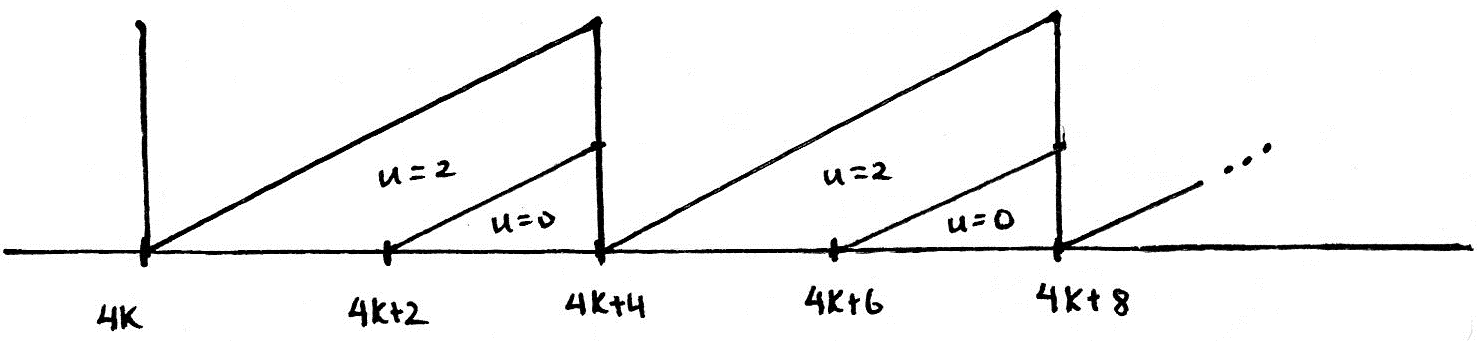
\includegraphics[scale=0.4]{./_Figures/f128img1.png}
\end{center}

Notice that characteristics crash immediately at $x(0) = 4k+2$ for $k \in \Z$. By the Rankine-Hugoniot condition, the shock curves are given by
$$ \dot{x}(t) = \frac{f(u_l) - f(u_r)}{u_l-u_r} = \frac{\frac{1}{2}(2)^2}{2} = 1, \quad x(0) = 4k+2 \quad \implies \quad x(t) = t+4k+2$$
\newpage
Hence, so far, we have the following picture:

\begin{center}
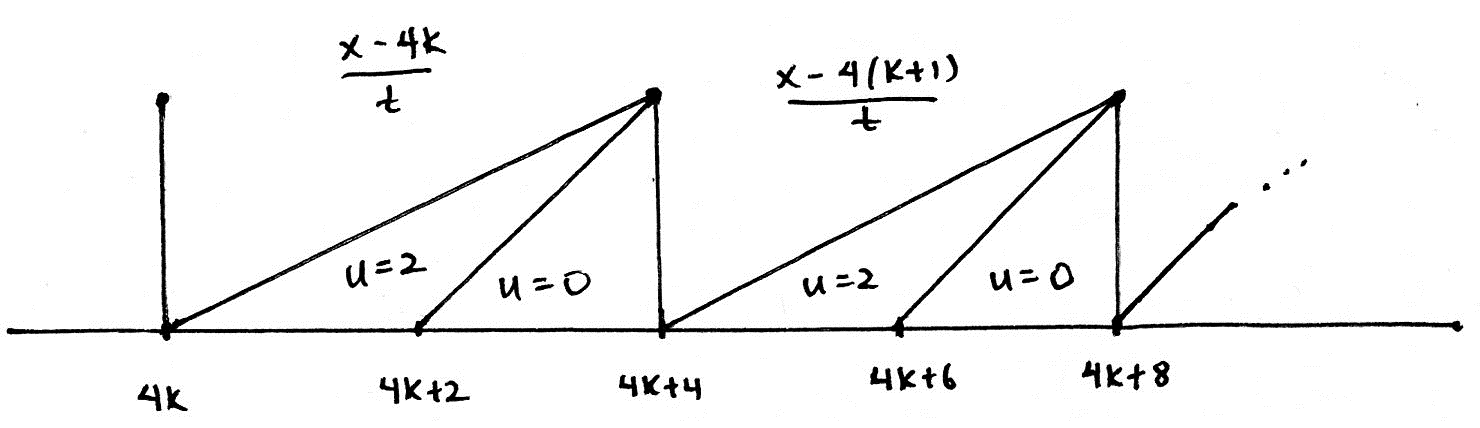
\includegraphics[scale=0.4]{./_Figures/f128img2.png}
\end{center}

Now, we fill in the regions $ \left\{ 4k < x < 4k+2t \right\}$ with rarefaction waves, which we define as $u = \frac{x-4k}{t}$. However, the characteristics $x = 4k+2t$ crash into the characteristics $x=4(k+1)$, which forms new shock curves. By Rankine-Hugoniot, these shocks are defined by
$$ \dot{x}(t) = \dfrac{\frac{1}{2} \left( \frac{x-4k}{t} \right)^2 - \frac{1}{2} \left( \frac{x-4(k+1)}{t} \right)^2}{\frac{x-4k}{t} - \frac{x-4(k+1)}{t}}, \quad x(2) = 4(k+1) $$
for $k \in \Z$. Solving this yields $x = t + 4k + 2$. Hence, our solution satisfies the following picture:

\begin{center}
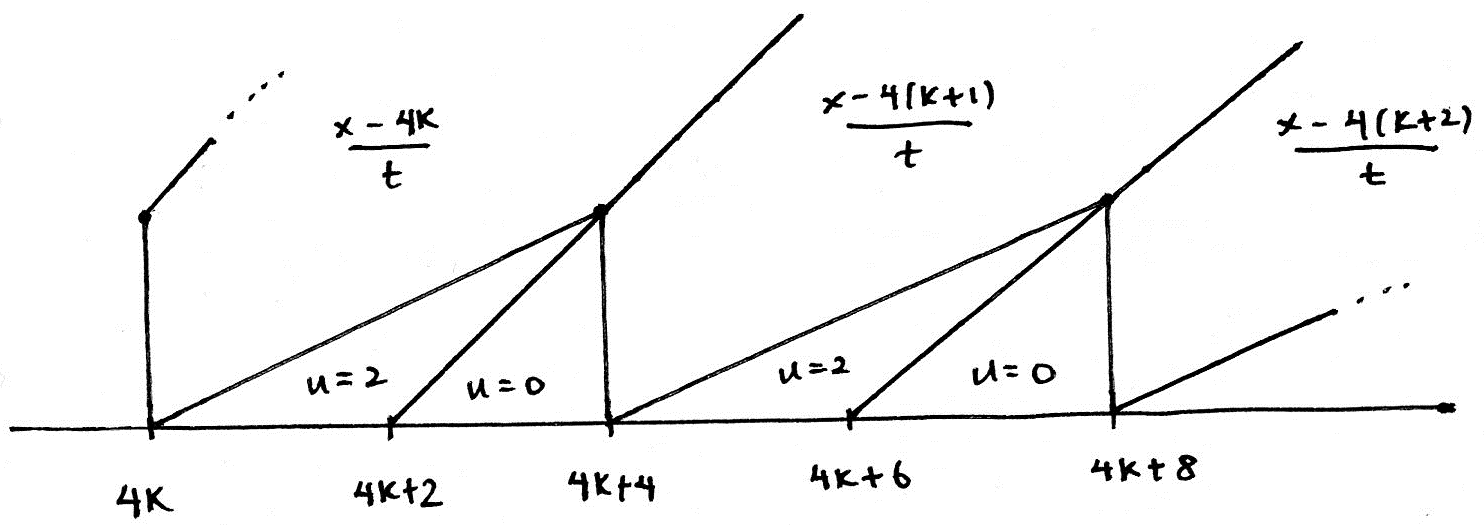
\includegraphics[scale=0.4]{./_Figures/f128img3.png}
\end{center}

Therefore, the slope of the solution, $\frac{\d u}{\d x}$, is $\frac{1}{t}$ almost everywhere for $t>2$. \hfill \qed
